\chapter{Synchronization System Case Study}
\label{chap:synchronization}

The main focus of this chapter is on a practical comparison between serverless and monolithic system implementations, specifically in the context of a synchronization system for a store's logistics system and its Shopify store, simulated by two servers, PS and SH respectively.

\section{System Overview}

The synchronization system is designed to maintain a consistent state between the store's logistics system and the Shopify store. It ensures that for every Item on PS, there exists an equivalent Variant on SH and that it is up-to-date, with PS being the source of truth. The synchronization task is mainly encapsulated in a single function, \texttt{syncModel(modelCode: String)}, which is deployed as an action on OpenWhisk in the serverless implementation and exposed as a route in the monolithic version.

API clients encapsulate CRUD operations for PS and SH. They handle operations such as fetching and updating items or stocks on PS and managing products, variants, and stocks on SH. 

\section{Experimental Setup}

The experimental setup involved deploying the monolithic and serverless implementations on machines of type m510 on CloudLab in the Utah cluster. Benchmarks were conducted using increasing workloads to assess the performance of each system. A custom-built rate limiter was used to control the flow of requests to the systems.

\section{Results and Discussion}

In comparison, the serverless implementation showed significantly slower performance, ranging from 4 to 10 times slower than the monolithic one. Even when using the rate limiter set at 70ms, the serverless implementation took 120ms, significantly slower than the monolithic implementation, which took 25ms.

\begin{figure}[h!]
    \centering
    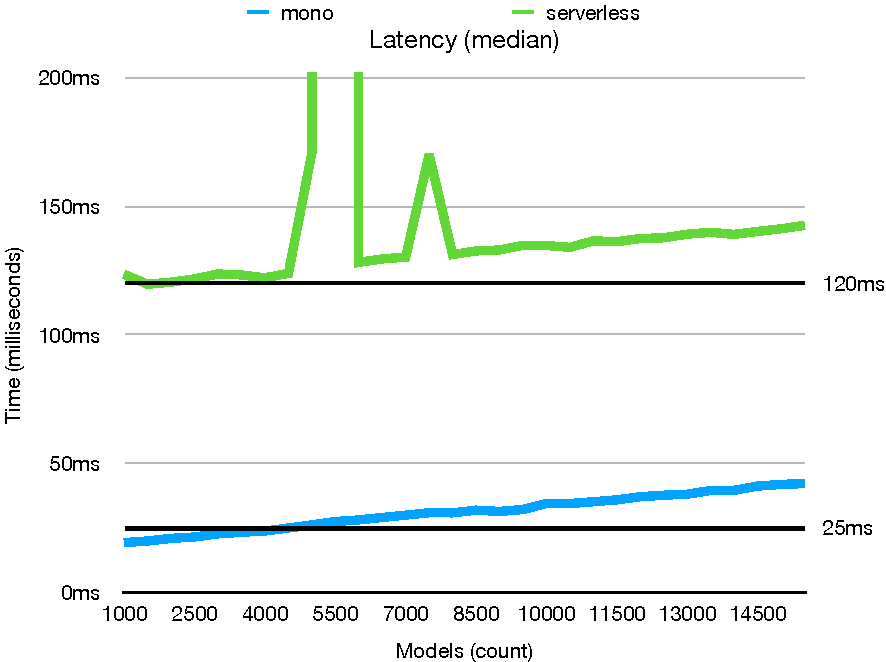
\includegraphics[width=\textwidth]{rate_l70ms_latency_med.pdf}
    \caption{Rate-limited comparison between serverless and monolithic implementations}
    \label{fig:rate_limited_comparison}
\end{figure}

Despite utilizing 18 machines for executing actions, the serverless approach did not show any clear benefits. This may be attributed to the lack of support for "intra-concurrency" in OpenWhisk runtimes, excluding NodeJS. This limitation significantly affects the scaling capabilities of the serverless implementation, which is a crucial aspect of the serverless or FaaS promise.

\section{Improvements and Future Work}

There are potential avenues for improvement in the serverless system. Notably, updating the Go proxy used by all OpenWhisk runtimes to support intra-concurrency could allow all language runtimes, including Swift, to support it, potentially reducing the execution latency. 

\section{Conclusion}

The case study findings contribute to the overall conclusion of this thesis, suggesting that the benefit of migrating to a serverless implementation is not always evident and should be carefully assessed for each workflow. The case study also highlights the importance of runtime support for intra-concurrency in realizing the full potential of serverless systems. Notably, the Swift runtime was updated to the latest version to leverage its native async/await features, which played a significant role in the serverless implementation.

\end{document}

